\section{University}
\Warning{}
%Since the address of the university corresponds to the address of who does the initial deploy, to login you need only to click on \emph{\textbf{Login}} at the top right of the screen.

%Once you've done this, 
After the login you will be redirected to the page represented in Figure~\ref{fig:loggedProfile}. As you can see, a black bar has appeared near the top of the screen.
The black bar contains on its left the voices \textbf{Academic Years}, \textbf{Degree Courses} and \textbf{Didactic activities}. On the right it contains the voices \textbf{Administrators}, \textbf{Professors} and \textbf{Students}.
The voices on the right allows the university to manage (create, visualize and delete) administrators, professors and students.

\begin{figure}[!h]
\centering
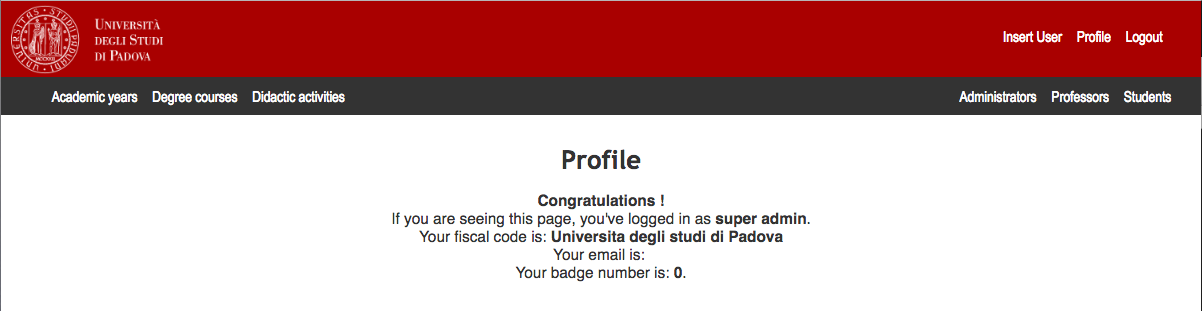
\includegraphics[width=0.65\textwidth]{img/loggedProfile.png}
\caption{Login with University}
\label{fig:loggedProfile}
\end{figure}

\subsection{Academic years}
By clicking on the \textbf{Academic years} voice in the menu, you will see (as in Figure~\ref{fig:acadYear}) a register of all the academic years inserted in the system. For each academic year you can \emph{insert a degree course}, \emph{modify the name of the academic year} and \emph{delete the academic year}.

\begin{figure}[!h]
  \centering
  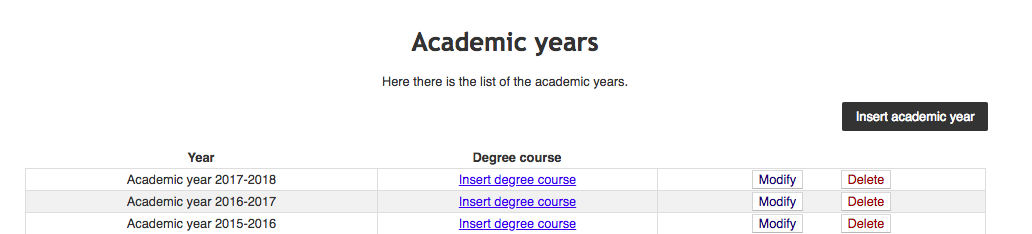
\includegraphics[width=0.90\textwidth]{img/accademicYears.png}
  \caption{Register of the the academic years registered in the system.}
  \label{fig:acadYear}
\end{figure}

\subsubsection{Insertion of a degree course}
Click on \textbf{Insert degree course}, you will be redirected to a page (like the one in Figure~\ref{fig:degreeInsertion}), insert the name of the degree course that you want to add and click the \textbf{save} button.
\begin{figure}[!h]
  \centering
  
\includegraphics[width=0.65\textwidth]{img/degreeInsertion.png}
  \caption{Insertion of a degree course.}
  \label{fig:degreeInsertion}
\end{figure}

\subsubsection{Modify the name of the academic year}
Click on the button \textbf{Modify}, you will be redirected to a page like the one in Figure~\ref{fig:modifyAcademicYear}, change the name
of the academic year and click the \textbf{save} button.
\begin{figure}[!h]
  \centering
  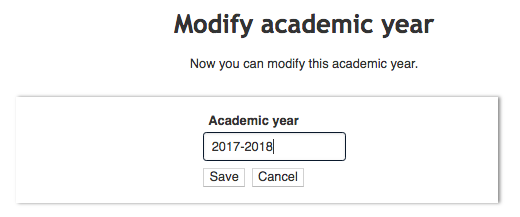
\includegraphics[width=0.65\textwidth]{img/modifyAcademicYear.png}
  \caption{Modification of an academic year.}
  \label{fig:modifyAcademicYear}
\end{figure}

\subsubsection{Elimination of an academic year}
Click on the button \textbf{Delete}, you will be redirected to a page (like the one in Figure~\ref{fig:deleteAcademicYear}) and click the \textbf{Delete} button to confirm the elimination.
\begin{figure}[!h]
  \centering
  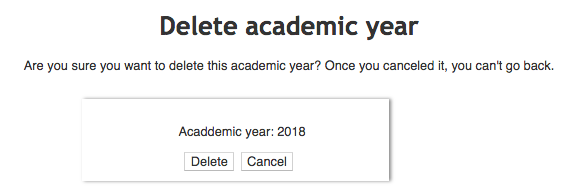
\includegraphics[width=0.65\textwidth]{img/deleteAcademicYear.png}
  \caption{Elimination of an academic year.}
  \label{fig:deleteAcademicYear}
\end{figure}

\subsection{Degree courses}
By clicking on the \textbf{Degree courses} voice in the menu, you will see (as in Figure~\ref{fig:degreeCourses}) a register of all the academic years inserted in the system for a specific academic year. For each degree course you can \emph{insert a didactic activity}, \emph{modify the name of the degree} and \emph{delete it}. 
\begin{figure}[!h]
  \centering
  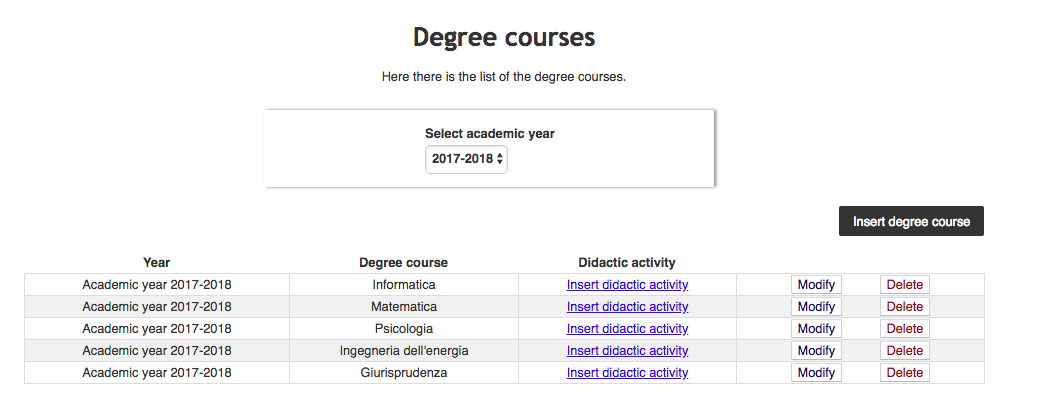
\includegraphics[width=0.90\textwidth]{img/degreeCourses.png}
  \caption{Register of the admins in the system.}
  \label{fig:degreeCourses}
\end{figure}

\subsubsection{Insert a didactic activity}
Click on the link \textbf{Insert didactic activity}, you will be redirected to a page like the one in Figure~\ref{fig:insertDidacticActivity}. You can insert the name of the activity, and also \emph{insert an exam} related to it by clicking on the link \textbf{Insert an exam}.
\begin{figure}[!h]
  \centering
  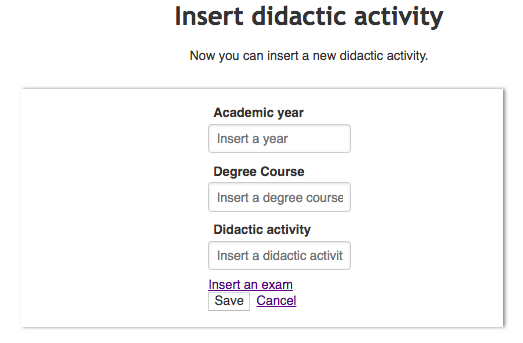
\includegraphics[width=0.70\textwidth]{img/insertDidacticActivity.png}
  \caption{Insertion of a didactic activity.}
  \label{fig:insertDidacticActivity}
\end{figure}

\subsubsection{Modify the name of a degree}
%%chiedere per anno accademico
Click on the button \textbf{Modify}, you will be redirected to a page like the one in Figure~\ref{fig:modifyDegree}, change the name
of the degree and click the \textbf{save} button.
\begin{figure}[!h]
  \centering
  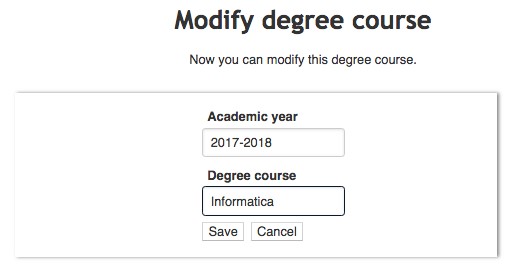
\includegraphics[width=0.65\textwidth]{img/modifyDegree.png}
  \caption{Modification of a degree.}
  \label{fig:modifyDegree}
\end{figure}

\subsubsection{Delete a degree}
Click on the link \textbf{Insert didactic activity}, you will be redirected to a page (like the one in Figure~\ref{fig:deleteDegree}). You can insert the name of the activity, and also \emph{insert an exam} related to it by clicking on the link \textbf{Insert an exam}.
\begin{figure}[!h]
  \centering
  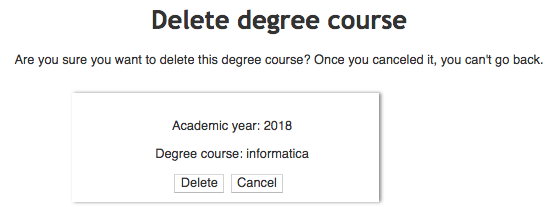
\includegraphics[width=0.65\textwidth]{img/deleteDegree.png}
  \caption{Elimination of a degree.}
  \label{fig:deleteDegree}
\end{figure}

\subsection{Didactic activities}
\WarningSubsection
\subsubsection{Insert an exam}
\WarningSubsection
\subsubsection{Modify a didactic activity}
\WarningSubsection
\subsubsection{Delete a didactic activity}
\WarningSubsection

\subsection{Administrators, Professors and Students management}
When you choose one of those three categories, you will see (as in Figure~\ref{fig:adminList}) a register of all its users listed by their 
name, surname, badge number, fiscal code and univocal code. You can choose to eliminate one of the listed users simply by clicking on the delete button corresponding to the user. 
\begin{figure}[!h]
  \centering
  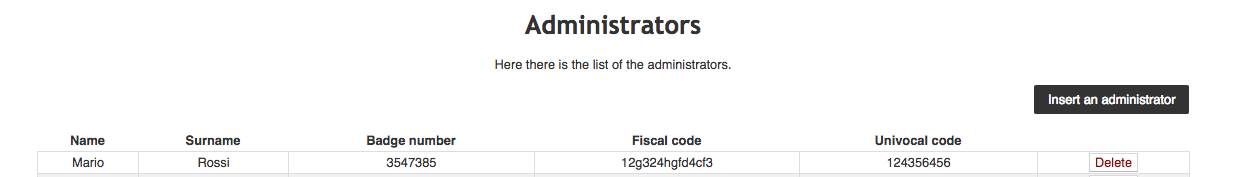
\includegraphics[width=0.90\textwidth]{img/adminList.png}
  \caption{Register of the admins in the system.}
  \label{fig:adminList}
\end{figure}


\section{Administrators}
An administrator has the same privileges of the university user but he can't create new administrator users.





